\chapter{Introduction} \label{introduction} 

The purpose of this research is to contribute in the diverse forms of use of the interactive learning environments by proposing a learning environment, we based the content management with an adaptive hypermedia approach and 
with the development of a new type of learning object to be adapted to the learning environment.
This environment use various devices that were capable of running a web browser, non-relational data bases for information exchange and some sensors like cameras and Kinect 2 were used. In addition we implemented a way to predict the level of user attention
which it was compared against information obtained by a video taken from the user doing the activity.

\section{Motivation}
There are many types of learning environments starting from the most basic that exist almost from the beginning of civilization where a person is able to learn based on their current context.
For example the first humans who needed to hunt them could take decisions and adapt to the situation and perform the task that was to hunt an animal to obtain food, in more recent times we can relate to the classrooms of schools, and currently including technology these Environments can be configurable and adapt to a particular context (the user).When a user uses learning environments the themes are usually flat and have the same content for everyone. In addition, users think and assimilate information in a different way which makes it more attractive to have a learning environment that adapts to the learning styles of the users and why not to the user preferences.

Nowadays most interactive museums work stations or exhibits like we see on the figure 1.1, where users come to the station to interact with or receive information by reversing some time on it until it passes to the next station, where the display will probably showed relevant information for the person but if this information is not shown to digestible way (processed so that it is attractive to the user) the user will probably spend less time or not time at all at the station. This expose the lack of adaptation of the exhibits in some interactive museums or standard museums. in order to ensure that the information and how is presented to the user is broadly engaging. 
\begin{figure}[ht!]  
\centering  
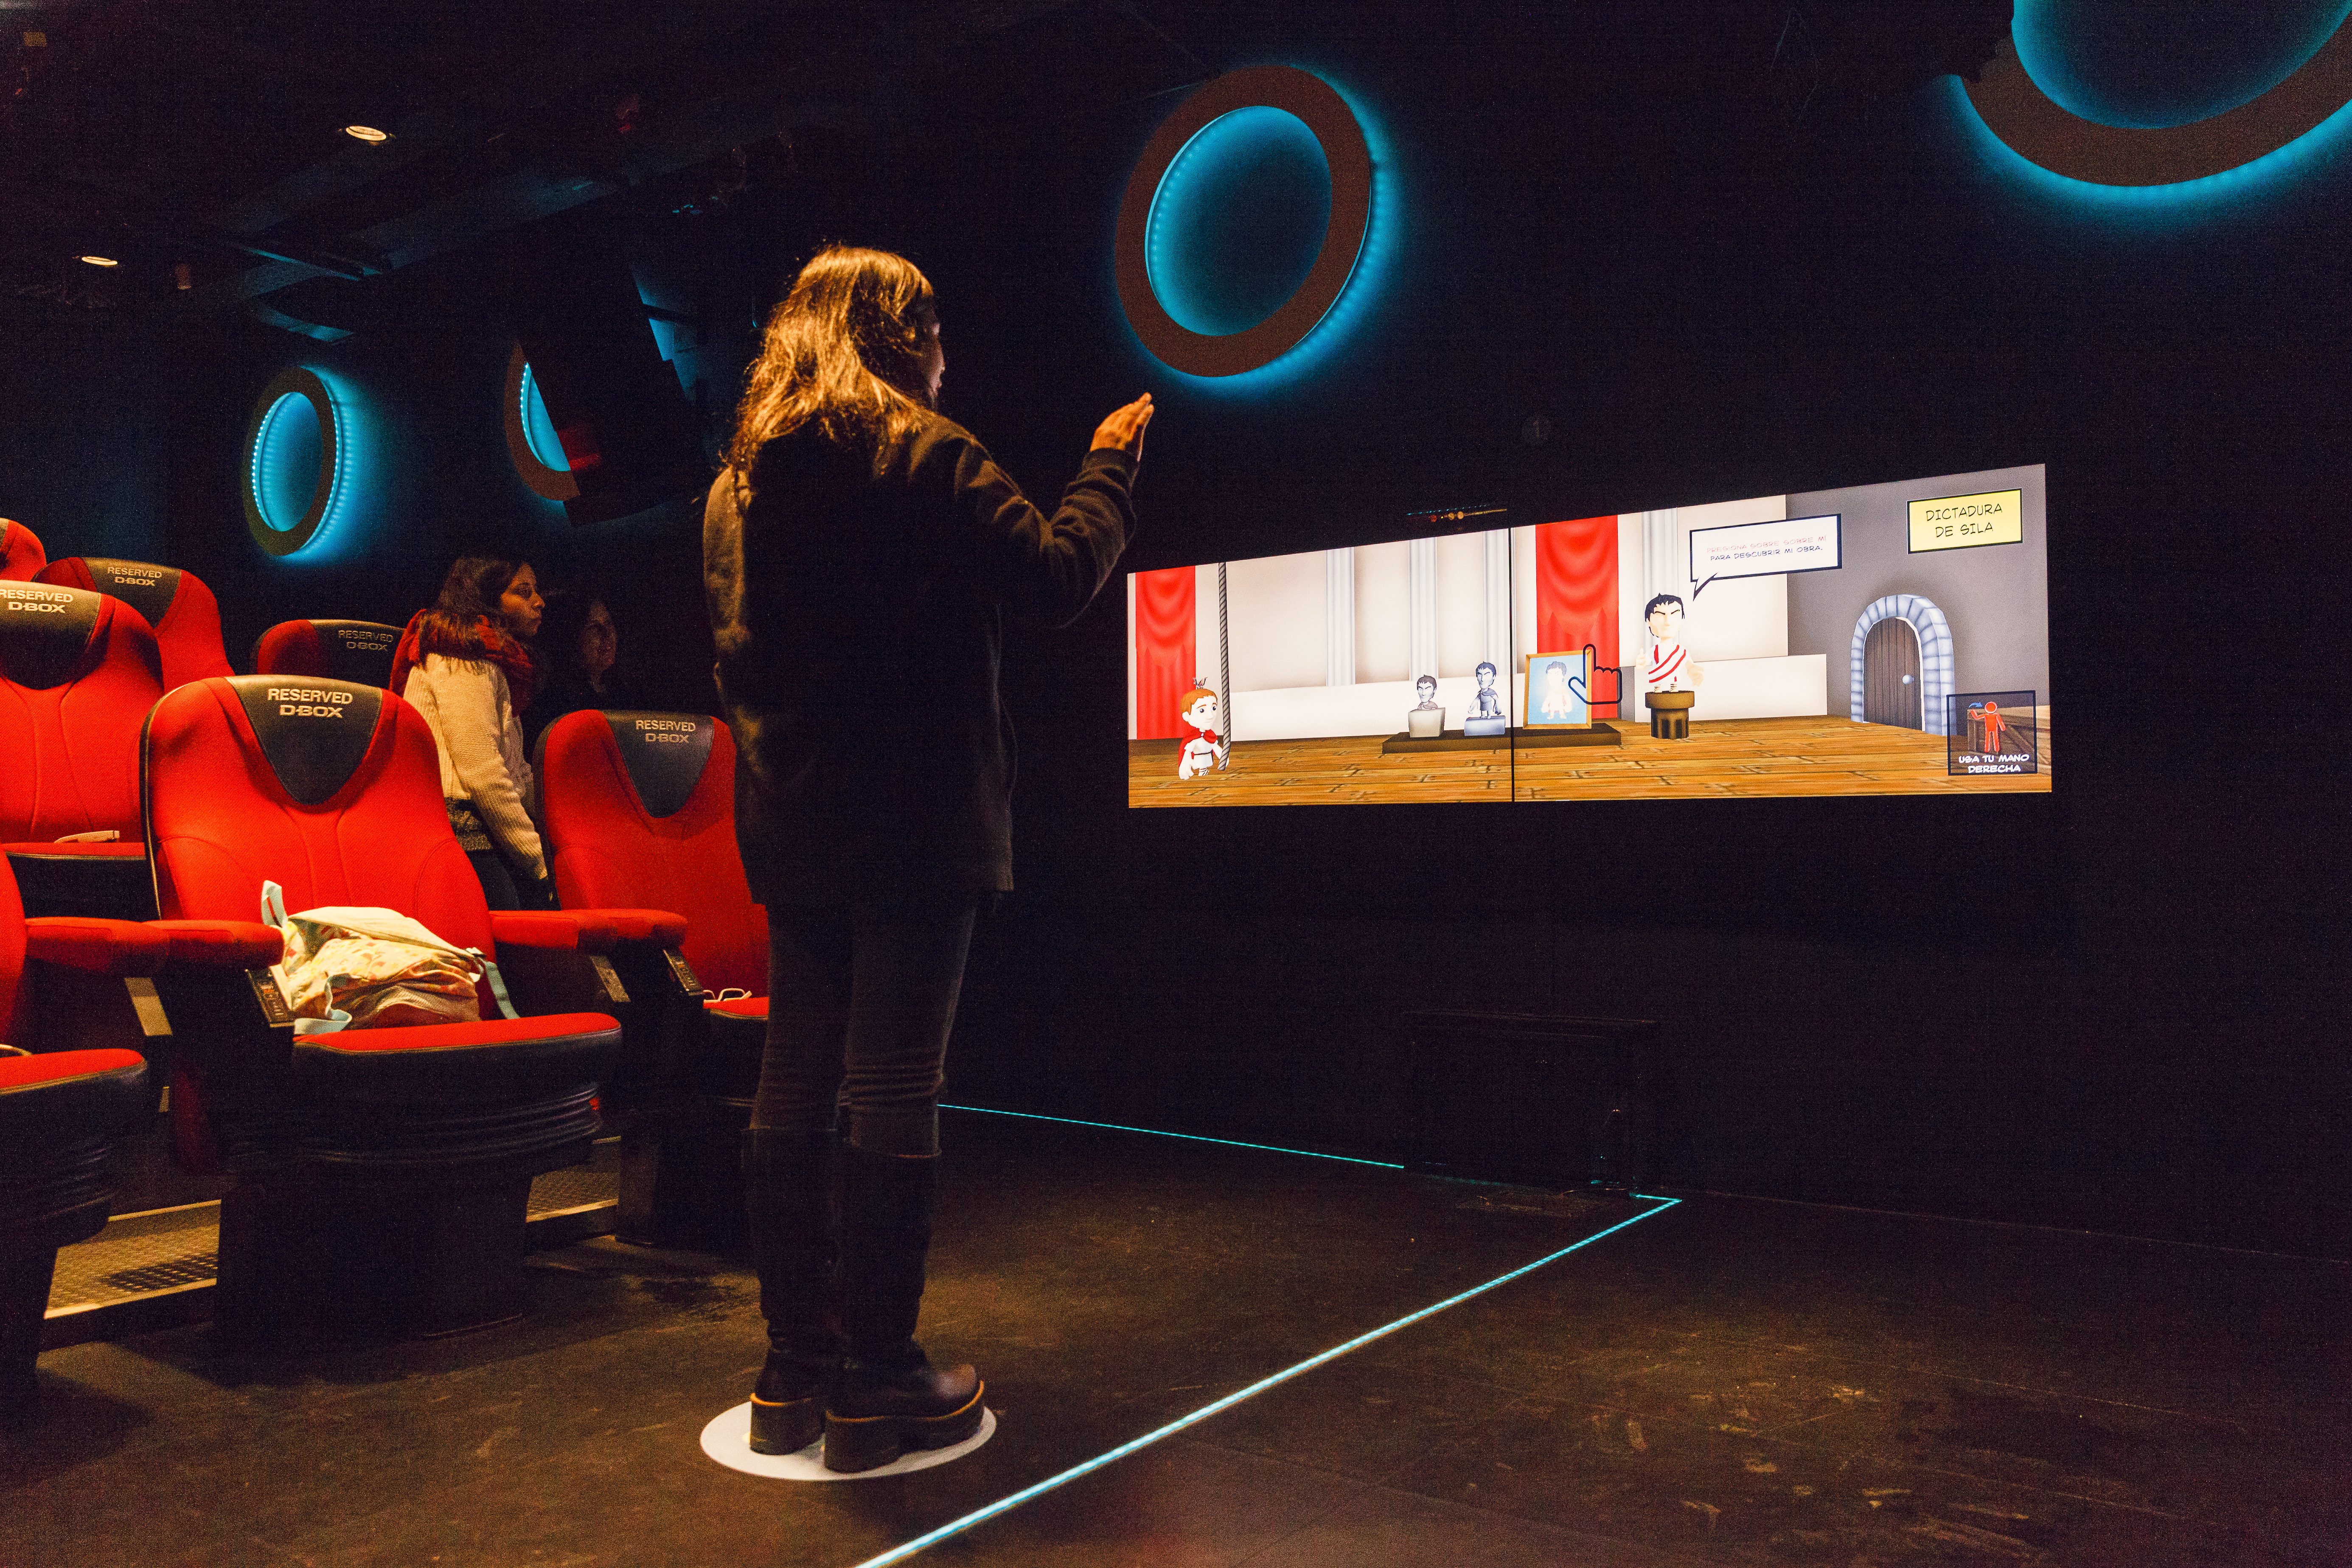
\includegraphics[scale=0.05]{musint}
\quad  
\caption{A museum interactive station}  
\label{name}  
\end{figure}
Intelligent learning environments can be used as exhibitors in museums they use embedded systems, sensors, information and communication technologies that are becoming invisible to the user as they are being integrated into physical objects, infrastructure, the environment in which we live, work and many other environments. This idea provides a good way of bridging the gap between human users and computing systems, and this motivates related research into Computing. Some of these systems use learning resources called learning objects. For the ex-change of learning objects between systems standardization initiatives have been developed and there are some implementations and repositories that manage the content using these standards. 

\section{Learning Environment}

The Learning Environment (LE) corresponds to the spaces in which the learning activities are developed, can be of three types: aulic, real and virtual. In the first it is the whole environment surrounding the student, in the context of the classroom, which focuses not only on the student, but also on the content, so the interaction with the environment will develop an interaction with the student that can be positive or negative depending the place. And has the following characteristics: 
\begin{itemize}
 \item The educator is the one who has to look for the models appropriate to their materials and the conditions of their group.
 \item They help to relate the content in an experimental and experiential way.
 \item It can be given a dynamic spatial distribution, changing as the group and the teacher consider it necessary.
\end{itemize}

The real Teaching-Learning activities are developed in the classroom, the real environment can be a laboratory, a company, clinic, library, green areas, etc. Real scenarios where you can see the application of knowledge and skills acquired, as well as the practice of attitudes and values. 

Virtual environments are those created through the use of Information and Communication Technologies, in order to provide learners with resources that facilitate their learning process, within these TICs can be cited the computer, cannon, a classroom Virtual, the use of internet where they can have access to blogs, discussion forums, chat, specialized pages where young people find fun activities, stories like solution to crosswords, puzzles, etc., that well employees contribute greatly in:
\begin{itemize}	
\item Acquisition of learning by the student.
\item Understand the nature and philosophy of distance education.
\item Identify the characteristics of students in remote locations.
\item Design and develop interactive materials that are adapted to the technology to be used, to the content, strategies and to facilitate independent study.
\end{itemize}
Learning environments are important in the day-to-day lives of people because we are in contact with them all the time in accordance with Phillips\cite{PhilMcNaKenn2010zx} a Learning Environment is a place where resources, time and reasons are available for a group of people to nurture, support and value the learning of a limited set of information. The LE are social places even when only one person is found there. 



One of the challenges facing the design of learning environments is human complexity, because each person thinks and assimilate information in different ways making it difficult to identify which resources are adequate for everyone. Intelligent learning environments (ILE) are a new type of intelligent educational system, which combines characteristics of traditional intelligent tutoring systems (ITS) \cite{john1991} and learning environments. According to Self \cite{self1998} ITS are learning systems based on computers that try to adapt to the needs of the learner. 
\begin{figure}[ht!]  
\centering  
\includegraphics[scale=1]{pizzarra}
\quad  
\caption{A kid using and intelligent chalk-board}  
\label{name}  
\end{figure}



\section{Learnign Objects.}
\section{Aim's.}
\section{Outline.}